\chapter{Limits}

%%% choose an epigraph to go here

\section{Encoding genealogies}

\subsection{The genealogical process}
Before we can analyse genealogies, we need a way to encode them.
The encoding will only include the information relevant to the sample genealogy, namely which lineages coalesce at which times. Information about particle positions and ``killed'' particles is ignored.

Let $\mathcal{P}_n$ be the space of partitions on $\{1,\dots,n\}$.
For convenience, we now label time in reverse, so the terminal particles are at time 0, their parents are at time 1, and so on.
Consider a sample of $n$ terminal particles among a total of $N$ particles, and label the sampled particles $1,\dots,n$.
The genealogical process $(G_t^{(n,N)})_{t\in\mathbb{N}_0}$ for this sample is the $\mathcal{P}_n$-valued stochastic process such that labels $i$ and $j$ are in the same block of the partition $G_t^{(n,N)}$ if and only if terminal particles $i$ and $j$ have a common ancestor at time $t$ (i.e.\ $t$ generations back).

A formulation where $G_t^{(n,N)}$ takes values in the space of equivalence relations from $[n]$ to $[n]$ is sometimes used; interpreting partition blocks as equivalence classes, this formulation is equivalent to ours.

The initial (time 0) value of the process is the partition of singletons $G_0^{(n,N)} = \{ \{1\}, \dots, \{n\} \}$, since all of the terminal particles are separate.
The only possible non-identity transitions are those that merge some blocks of the partition; this encodes the coalescence of the corresponding lineages.
The trivial partition $\{ \{1,\dots,n\} \}$ is therefore an absorbing state, corresponding to all lineages in the sample having coalesced (i.e.\ the MRCA has been reached).
The construction of the genealogical process from the resampling indices is illustrated in Figure \ref{fig:encoding_genealogy}.

\begin{figure}
\centering
\subfloat[Resampling relationships]{
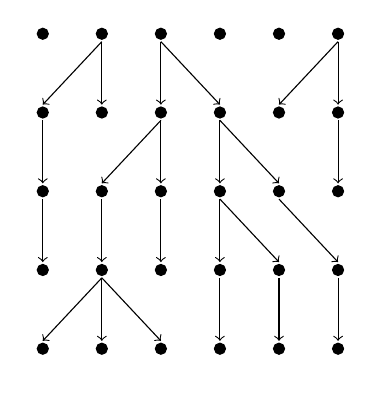
\begin{tikzpicture}
% grid of particles
\filldraw (0,0) circle (2pt);
\filldraw (0.75,0) circle (2pt);
\filldraw (1.5,0) circle (2pt);
\filldraw (2.25,0) circle (2pt);
\filldraw (3,0) circle (2pt);
\filldraw (3.75,0) circle (2pt);
\filldraw (0,1) circle (2pt);
\filldraw (0.75,1) circle (2pt);
\filldraw (1.5,1) circle (2pt);
\filldraw (2.25,1) circle (2pt);
\filldraw (3,1) circle (2pt);
\filldraw (3.75,1) circle (2pt);
\filldraw (0,2) circle (2pt);
\filldraw (0.75,2) circle (2pt);
\filldraw (1.5,2) circle (2pt);
\filldraw (2.25,2) circle (2pt);
\filldraw (3,2) circle (2pt);
\filldraw (3.75,2) circle (2pt);
\filldraw (0,3) circle (2pt);
\filldraw (0.75,3) circle (2pt);
\filldraw (1.5,3) circle (2pt);
\filldraw (2.25,3) circle (2pt);
\filldraw (3,3) circle (2pt);
\filldraw (3.75,3) circle (2pt);
\filldraw (0,4) circle (2pt);
\filldraw (0.75,4) circle (2pt);
\filldraw (1.5,4) circle (2pt);
\filldraw (2.25,4) circle (2pt);
\filldraw (3,4) circle (2pt);
\filldraw (3.75,4) circle (2pt);
% resampling arrows % generation 4 to 5
\draw[->] (0.75,0.9)--(0,0.1);
\draw[->] (0.75,0.9)--(0.75,0.1);
\draw[->] (0.75,0.9)--(1.5,0.1);
\draw[->] (2.25,0.9)--(2.25,0.1);
\draw[->] (3,0.9)--(3,0.1);
\draw[->] (3.75,0.9)--(3.75,0.1);
% resampling arrows % generation 3 to 4
\draw[->] (0,1.9)--(0,1.1);
\draw[->] (0.75,1.9)--(0.75,1.1);
\draw[->] (1.5,1.9)--(1.5,1.1);
\draw[->] (2.25,1.9)--(2.25,1.1);
\draw[->] (2.25,1.9)--(3,1.1);
\draw[->] (3,1.9)--(3.75,1.1);
% resampling arrows % generation 2 to 3
\draw[->] (0,2.9)--(0,2.1);
\draw[->] (1.5,2.9)--(0.75,2.1);
\draw[->] (1.5,2.9)--(1.5,2.1);
\draw[->] (2.25,2.9)--(2.25,2.1);
\draw[->] (2.25,2.9)--(3,2.1);
\draw[->] (3.75,2.9)--(3.75,2.1);
% resampling arrows % generation 1 to 2
\draw[->] (0.75,3.9)--(0,3.1);
\draw[->] (0.75,3.9)--(0.75,3.1);
\draw[->] (1.5,3.9)--(1.5,3.1);
\draw[->] (1.5,3.9)--(2.25,3.1);
\draw[->] (3.75,3.9)--(3,3.1);
\draw[->] (3.75,3.9)--(3.75,3.1);
% fudge bottom space
\node[anchor=north] at (0,0) {\textcolor{white}{\footnotesize{1}}};
\end{tikzpicture}
\label{fig:encoding_a}
}
\hspace{0.9cm}
\subfloat[Genealogy of terminal particles]{
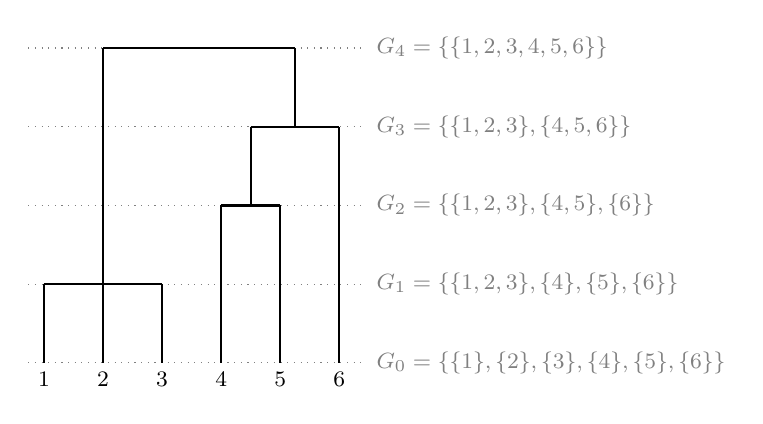
\begin{tikzpicture}
% horizontal time lines
\draw[gray,dotted] (-0.2,0)--(4.05,0);
\draw[gray,dotted] (-0.2,1)--(4.05,1);
\draw[gray,dotted] (-0.2,2)--(4.05,2);
\draw[gray,dotted] (-0.2,3)--(4.05,3);
\draw[gray,dotted] (-0.2,4)--(4.05,4);
% tree
\draw[thick] (0.75,0)--(0.75,4);
\draw[thick] (0,0)--(0,1);
\draw[thick] (1.5,0)--(1.5,1);
\draw[thick] (0,1)--(1.5,1);
\draw[thick] (2.25,0)--(2.25,2);
\draw[thick] (3,0)--(3,2);
\draw[thick] (2.25,2)--(3,2);
\draw[thick] (2.625,2)--(2.625,3);
\draw[thick] (3.75,0)--(3.75,3);
\draw[thick] (2.625,3)--(3.75,3);
\draw[thick] (3.1875,3)--(3.1875,4);
\draw[thick] (0.75,4)--(3.1875,4);
% lineage labels
\node[anchor=north] at (0,0) {\footnotesize{1}};
\node[anchor=north] at (0.75,0) {\footnotesize{2}};
\node[anchor=north] at (1.5,0) {\footnotesize{3}};
\node[anchor=north] at (2.25,0) {\footnotesize{4}};
\node[anchor=north] at (3,0) {\footnotesize{5}};
\node[anchor=north] at (3.75,0) {\footnotesize{6}};
% partition labels
\node[anchor=west] at (4.1,0) {\textcolor{gray}{\footnotesize{$G_0 = \{ \{1\}, \{2\}, \{3\}, \{4\}, \{5\}, \{6\} \}$}}};
\node[anchor=west] at (4.1,1) {\textcolor{gray}{\footnotesize{$G_1 = \{ \{1,2,3\}, \{4\}, \{5\}, \{6\} \}$}}};
\node[anchor=west] at (4.1,2) {\textcolor{gray}{\footnotesize{$G_2 = \{ \{1,2,3\}, \{4,5\}, \{6\} \}$}}};
\node[anchor=west] at (4.1,3) {\textcolor{gray}{\footnotesize{$G_3 = \{ \{1,2,3\}, \{4,5,6\} \}$}}};
\node[anchor=west] at (4.1,4) {\textcolor{gray}{\footnotesize{$G_4 = \{ \{1,2,3,4,5,6\} \}$}}};
\end{tikzpicture}
\label{fig:encoding_b}
}
\caption[Illustration of how the sample genealogy is encoded]{Illustration of how the sample genealogy is encoded. \subref{fig:encoding_a} Relationships induced by resampling with six particles over four iterations. \subref{fig:encoding_b} The genealogy of the terminal particles, labelled with the value of the genealogical process $G_t$ at each time.}
\label{fig:encoding_genealogy}
\end{figure}


\subsection{Time scale}
In order to get a continuous limit, we scale time by a function $\tau_N(\cdot)$. In the population genetics literature, a deterministic time scale can be used \seb{[citations] and/or this will have been mentioned already in pop gen example models (Section \ref{sec:popgenmodels})}, whereas in our case $\tau_N$ depends on the offspring counts and is therefore random.
To define the time scale we first define the pair merger rate
\begin{equation}\label{eq:defn_cN}
c_N(t) := \frac{1}{(N)_2} \sum_{i=1}^N (\nu_t^{(i)})_2 .
\end{equation}
This is the probability, conditional on $\nu_t^{(1:N)}$, that a randomly chosen pair of lineages in generation $t$ merges exactly one generation back.
To achieve the limiting pair merger rate of 1, as in the $n$-coalescent, we rescale time by the generalised inverse
\begin{equation}\label{eq:defn_tauN}
\tau_N(t) := \inf \left\{ s \geq 1 : \sum_{r=1}^s c_N(r) \geq t \right\} .
\end{equation}
The function $\tau_N$ maps continuous to discrete time, providing the link between the discrete-time SMC dynamics and the continuous-time Kingman limit.
We will also need the following quantity, which is an upper bound on the rate of multiple mergers (three or more lineages merging, or two or more simultaneous pairwise mergers):
\begin{equation}\label{eq:defn_DN}
D_N(t) := \frac{1}{N(N)_2} \sum_{i=1}^N (\nu_t^{(i)})_2
        \left\{ \nu_t^{(i)} + \frac{1}{N} \sum_{j\neq i} (\nu_t^{(j)})^2 \right\} .
\end{equation} 
%Let $\nu_t^{(i)}$ be the number of offspring in generation $t$ of particle $i$ ($t \in \mathbb{N}$, $i = 1,\dots, N$).
%Let $(\mathcal{F}_t)$ be the reverse-time filtration generated by the offspring counts.
Some basic properties are given in Proposition~\ref{thm:cN_properties}.
\begin{prop}[Properties of $c_N$]\label{thm:cN_properties}
For all $t\in\mathbb{N}$, $t^\prime > s^\prime >0$,
\begin{enumerate}[label=(\alph*)]
\item \label{item:cN_property1} \hspace{5pt}
    $\begin{aligned}
    c_N(t) , D_N(t) \in [0,1]
    \end{aligned}$
\item \label{item:cN_property2} \hspace{5pt}
    $\begin{aligned}
    D_N(t) \leq c_N(t)
    \end{aligned}$
\item \label{item:cN_property3} \hspace{5pt}
    $\begin{aligned}
    c_N(t)^2 \leq c_N(t) 
    \end{aligned}$
\item \label{item:cN_property4} \hspace{5pt}
    $\begin{aligned}
    t^\prime
    \leq \sum_{r=1}^{\tau_N(t^\prime)} c_N(r) 
    \leq t^\prime +1 .
    \end{aligned}$
\item \label{item:cN_property5} \hspace{5pt}
    $\begin{aligned}
    t^\prime - s^\prime -1
    \leq \sum_{r=\tau_N(s^\prime)+1}^{\tau_N(t^\prime)} c_N(r) 
    \leq t^\prime - s^\prime +1 .
    \end{aligned}$
\end{enumerate}
%\begin{align}
%& c_N(t) , D_N(t) \in [0,1] \label{eq:cN_property1}\\
%& D_N(t) \leq c_N(t) \label{eq:cN_property2}\\
%& c_N(t)^2 \leq c_N(t) \label{eq:cN_property3}\\
%& t^\prime \leq \sum_{r=1}^{\tau_N(t^\prime)} c_N(r) \leq t^\prime +1 . \label{eq:cN_property4}
%\end{align}
\end{prop}

\begin{proof}
\textbf{\ref{item:cN_property1}}  $c_N(t)$ and $D_N(t)$ are clearly non-negative. Both are maximised when one of the offspring counts is equal to $N$ and the rest are zero, in which case $c_N(t) = D_N(t) = 1$.\\
\textbf{\ref{item:cN_property2}} As outlined in \textcite[p.9]{koskela2018},
\begin{align*}
D_N(t) &:= \frac{1}{(N)_2} \sum_{i=1}^N (\nu_t^{(i)})_2 \frac{1}{N} \left\{  \nu_t^{(i)} + \frac{1}{N} \sum_{j\neq i}^N (\nu_t^{(j)})^2 \right\} \\
&\leq \frac{1}{(N)_2} \sum_{i=1}^N (\nu_t^{(i)})_2 \frac{1}{N} \left\{  \nu_t^{(i)} + \frac{1}{N} \sum_{j\neq i}^N N \nu_t^{(j)} \right\} \\
&= \frac{1}{(N)_2} \sum_{i=1}^N (\nu_t^{(i)})_2 \frac{1}{N} \left\{ \sum_{j =1}^N \nu_t^{(j)} \right\}
\leq \frac{1}{(N)_2} \sum_{i=1}^N (\nu_t^{(i)})_2
= c_N(t) .
\end{align*}
\textbf{\ref{item:cN_property3}} is immediate given \ref{item:cN_property1}.\\
\textbf{\ref{item:cN_property4}} follows directly from the definition of $\tau_N$ in \eqref{eq:defn_tauN}.\\
\textbf{\ref{item:cN_property5}} Writing
\begin{equation*}
\sum_{r=\tau_N(s^\prime)+1}^{\tau_N(t^\prime)} c_N(r)
= \sum_{r=1}^{\tau_N(t^\prime)} c_N(r) 
        - \sum_{r=1}^{\tau_N(s^\prime)} c_N(r) ,
\end{equation*}
the result follows by applying \ref{item:cN_property4} to both sums.
\end{proof}



\subsection{Transition probabilities}
\draft{Introduce $p_{\xi\eta}$. Present expression for that (or at least for $p_{\xi\xi}$), and hence the bounds on it that will be used later (keeping big-O terms explicit where possible).}

Let $\mathcal{P}_n$ be the space of partitions of $\{1,\dots,n\}$, and denote by $\Delta$ the partition of singletons $\{ \{1\},\dots, \{n\} \}$.
For any $\xi, \eta \in \mathcal{P}_n$ and $t\in\mathbb{N}$, let $p_{\xi\eta}(t)$ denote the conditional transition probabilities of the genealogical process given $\nu_t^{(1:N)}$ ($t\in\mathbb{N}$, $\xi, \eta \in \mathcal{P}_n$).
The transition probability $p_{\xi\eta}(t)$ can only be non-zero when $\eta$ can be obtained from $\xi$ by merging some blocks of $\xi$.
Ordering the blocks by their least element, denote by $b_i$ the number of blocks of $\xi$ that merge to form block $i$ in $\eta$ ($i \in \{1,\dots, |\eta|\}$). Hence $b_1 + \cdots + b_{|\eta|} = |\xi|$.
Then the transition probability is given by
\begin{equation}\label{eq:defn_pxieta}
p_{\xi\eta}(t) 
:= \frac{1}{(N)_{|\xi|}} \sum_{\substack{i_1 \neq \cdots \neq i_{|\eta|} \\ =1}}^N
        (\nu_t^{(i_1)})_{b_1} \cdots (\nu_t^{(i_{|\eta|})})_{b_{|\eta|}} .
\end{equation}
We will only need to work directly with the \emph{identity} transition probabilities $p_{\xi\xi}(t)$.
Upper and lower bounds on these probabilities are presented in Propositions \ref{thm:pDelta_LB} and \ref{thm:pDelta_UB}.
\begin{prop}[Lower bound on identity transition probabilities]\label{thm:pDelta_LB}
Let $\xi \in \mathcal{P}_n$, $N>2$. Then
\begin{equation*}
p_{\xi\xi}(t)
\geq 1 - \binom{|\xi|}{2} \frac{N^{n-2}}{(N-2)_{n-2}} \left[ c_N(t) + B_{|\xi|} D_N(t) \right]
\end{equation*}
where $B_{|\xi|} = K (|\xi|-1)! (|\xi|-2) \exp( 2 \sqrt{2(|\xi|-2)} )$ for some $K>0$ that does not depend on $|\xi|$.
\end{prop}
\seb{For weak convergence proof, refer to this proposition but rewrite the inequality using $\xi = \Delta$ and $\alpha_n$, to provide a local target for cross-referencing. Similarly for UB.}
\begin{proof}
%The proof follows \textcite[Proof of Lemma 3.6]{brown2021}, but keeping the terms in $N$ explicit. --- I don't need to refer to BJJK as it's part of my work; just reproduce BJJK's workings nice and verbosely here :)
We have the following expression for $p_{\xi\xi}(t)$, by subtracting all possible non-identity transitions (the omitted $k=|\xi|$ term would count identity transitions):
\begin{equation*}
p_{ \xi \xi }( t ) 
= 1 - \frac{ 1 }{ ( N )_{ | \xi | } } \sum_{ k = 1 }^{ | \xi | - 1 } 
        \sum_{ \substack{ b_1 \geq \ldots \geq b_k = 1 
        \\ b_1 + \ldots + b_k = | \xi | } }^{ | \xi | } 
        \frac{ | \xi |! }{ \prod_{ j = 1 }^{ | \xi | } ( j ! )^{ \kappa_j } \kappa_j ! } 
        \sum_{ \substack{ i_1 \neq \ldots \neq i_k = 1 \\ \text{all distinct} } }^N 
        ( \nu_t^{ ( i_1 ) } )_{ b_1 } \ldots ( \nu_t^{ ( i_k ) } )_{ b_k },
\end{equation*}
where $\kappa_i = |\{ j : b_j = i \}|$ is the multiplicity of mergers of size $i$ ($\kappa_1$ counts non-merger events, and we have the identity $\kappa_1 + 2 \kappa_2 + \cdots + | \xi | \kappa_{ | \xi | } = | \xi |$).
The combinatorial factor is the number of partitions of a sequence of length $|\xi|$  having $\kappa_j$ subsequences of length $j$ for each $j$ \parencite[Equation (11)]{fu2006}.

We separate the $k=|\xi|-1$ term (which counts single pair mergers), for which $(b_1, b_2, \dots, b_{|\xi|-1}) = (2,1,\dots,1)$ and
\begin{equation*}
\frac{ | \xi |! }{ \prod_{ j = 1 }^{ | \xi | } ( j ! )^{ \kappa_j } \kappa_j ! }
= \binom{|\xi|}{2} .
\end{equation*}
For the remaining terms we use
\begin{equation*}
\frac{ | \xi |! }{ \prod_{ j = 1 }^{ | \xi | } ( j ! )^{ \kappa_j } \kappa_j ! }
\leq |\xi|! .
\end{equation*}
Thus
\begin{align*}
p_{ \xi \xi }( t ) 
&\geq 1 - \frac{ 1 }{ ( N )_{ | \xi | } } \binom{|\xi|}{2}
        \sum_{ \substack{ i_1 \neq \ldots \neq i_{|\xi|-1} = 1 \\ \text{all distinct} } }^N 
        ( \nu_t^{ ( i_1 ) } )_2 \nu_t^{(i_2)} \ldots \nu_t^{ ( i_{|\xi|-1} ) } \\
    &\qquad- \frac{ 1 }{ ( N )_{ | \xi | } } \sum_{ k = 1 }^{ | \xi | - 1 } 
        \sum_{ \substack{ b_1 \geq \ldots \geq b_k = 1 
        \\ b_1 + \ldots + b_k = | \xi | } }^{ | \xi | } |\xi|!
        \sum_{ \substack{ i_1 \neq \ldots \neq i_k = 1 \\ \text{all distinct} } }^N 
        ( \nu_t^{ ( i_1 ) } )_{ b_1 } \ldots ( \nu_t^{ ( i_k ) } )_{ b_k }
\end{align*}
Now, for the $k=|\xi|-1$ term we use the bound
\begin{equation*}
\sum_{ i_1 \neq \ldots \neq i_{ | \xi | - 1 } = 1 }^N 
        ( \nu_t^{ ( i_1 ) } )_2 \nu_t^{ ( i_2 ) } \ldots \nu_t^{ ( i_{ | \xi | - 1 } ) }
\leq N^{ | \xi | - 2 } \sum_{ i = 1 }^N ( \nu_t^{ ( i ) } )_2
\end{equation*}
while for the other terms we have \parencite[similarly to][Lemma 1 Case 3]{koskela2018}
\begin{align*}
\sum_{ \substack{ i_1 \neq \ldots \neq i_k = 1 \\ \text{all distinct} } }^N &( \nu_t^{ ( i_1 ) } )_{ b_1 } \ldots ( \nu_t^{ ( i_k ) } )_{ b_k } \leq \sum_{ i = 1 }^N ( \nu_t^{ ( i ) } )_2 \Bigg( N^{ | \xi | - 2 } - \sum_{ \substack{ j_1 \neq \ldots \neq j_{ | \xi | - 2 } = 1 \\ \text{all distinct and } \neq i } }^N \nu_t^{ ( j_1 ) } \ldots \nu_t^{ ( j_{ | \xi | - 2 } ) } \Bigg) \\
&\leq \sum_{ i = 1 }^N ( \nu_t^{ ( i ) } )_2 \Bigg\{ N^{ | \xi | - 2 } - ( N - \nu_t^{ ( i ) } )^{ | \xi | - 2 } + \binom{ | \xi | - 2 }{ 2 } \sum_{ j \neq i } ( \nu_t^{ ( j ) } )^2 \Bigg( \sum_{ k \neq i } \nu_t^{ ( k ) } \Bigg)^{ | \xi | - 4 } \Bigg\} \\
&\leq \sum_{ i = 1 }^N ( \nu_t^{ ( i ) } )_2 \Bigg\{ ( | \xi | - 2 ) \nu_t^{ ( i ) } N^{ | \xi | - 3 } + \binom{ | \xi | - 2 }{ 2 } \sum_{ j \neq i } ( \nu_t^{ ( j ) } )^2 N^{ | \xi | - 4 } \Bigg\},
\end{align*}
where the last step uses $(N - x)^b \geq N^b - b x N^{ b - 1 }$ for $x \leq N$, $b \geq 0$.
Hence
\begin{align*}
p_{ \xi \xi }( t ) 
&\geq 1 - \frac{ 1 }{ ( N )_{ | \xi | } } \binom{|\xi|}{2}
        N^{ | \xi | - 2 } \sum_{ i = 1 }^N ( \nu_t^{ ( i ) } )_2 \\
    &\qquad- \frac{ N^{|\xi|-3} }{ ( N )_{ | \xi | } } |\xi|!
        \sum_{ k = 1 }^{ | \xi | - 1 } 
        \sum_{ \substack{ b_1 \geq \ldots \geq b_k = 1 
        \\ b_1 + \ldots + b_k = | \xi | } }^{ | \xi | } 
        \sum_{ i = 1 }^N ( \nu_t^{ ( i ) } )_2 
        \Bigg\{ ( | \xi | - 2 ) \nu_t^{ ( i ) } + \binom{ | \xi | - 2 }{ 2 } \frac{1}{N} 
        \sum_{ j \neq i } ( \nu_t^{ ( j ) } )^2 \Bigg\} .
\end{align*}
The summands in the last line are independent of $k, b_i$, and the number of terms in the sums over $k$ and $b_1, \dots, b_k$ is bounded by $\gamma_{|\xi|-2} (|\xi|-2)$, where $\gamma_n$ is the number of integer partitions of $n$.
By \textcite[Section 2]{hardy1918}, $\gamma_n < K e^{ 2 \sqrt{ 2 n } } / n$ for a constant $K > 0$ independent of $n$.
Thus, for $|\xi| > 2$,
\begin{align*}
p_{ \xi \xi }( t ) 
&\geq 1 - \frac{ N^{ | \xi | - 2 } }{ ( N-2 )_{ | \xi | -2} } \binom{|\xi|}{2}
        c_N(t) \\
    &\qquad- \frac{ N^{|\xi|-2} }{ ( N-2 )_{ | \xi | -2} }
        K \exp( 2 \sqrt{2(|\xi|-2)} ) |\xi|!
        \frac{1}{N(N)_2} \\
    &\hspace{4cm} \sum_{ i = 1 }^N ( \nu_t^{ ( i ) } )_2
        \Bigg\{ ( | \xi | - 2 ) \nu_t^{ ( i ) } + \binom{ | \xi | - 2 }{ 2 } \frac{1}{N} 
        \sum_{ j \neq i } ( \nu_t^{ ( j ) } )^2 \Bigg\} \\
&\geq 1 - \frac{ N^{ | \xi | - 2 } }{ ( N-2 )_{ | \xi | -2} } \binom{|\xi|}{2}
        c_N(t) \\
    &\qquad- \frac{ N^{|\xi|-2} }{ ( N-2 )_{ | \xi | -2} }
        K \exp( 2 \sqrt{2(|\xi|-2)} ) |\xi|! \binom{ |\xi|-1}{2} D_N(t) \\
&\geq 1 - \frac{ N^{ | \xi | - 2 } }{ ( N-2 )_{ | \xi | -2} } \binom{|\xi|}{2}
        \left[ c_N(t) + B_{|\xi|} D_N(t) \right]
\end{align*}
where
\begin{align*}
B_{|\xi|} 
&= \binom{|\xi|}{2}^{-1} K \exp( 2 \sqrt{2(|\xi|-2)} ) |\xi|! \binom{ |\xi|-1}{2} \\
&= K (|\xi|-1)! (|\xi|-2) \exp( 2 \sqrt{2(|\xi|-2)} ) .
\end{align*}
When $|\xi| \leq 2$, there are no terms with $k\leq |\xi|-2$, and the result is immediate.
\end{proof}


\begin{prop}[Upper bound on identity transition probabilities]\label{thm:pDelta_UB}
Let $\xi \in \mathcal{P}_n$, $N>...$ \seb{it came out as $N\geq n^2(n-3)+1$ for the $\xi=\Delta$ case, up to possible errors}. Then
\begin{equation*}
p_{\xi\xi}(t)
\leq 1 - \binom{|\xi|}{2} \frac{N^{n-2}}{(N-2)_{n-2}} 
        \left[ c_N(t) - B_{|\xi|}^\prime D_N(t) \right]
\end{equation*}
where $B_{|\xi|}^\prime = ...$.
\end{prop}

\begin{proof}
The proof follows \textcite[Proof of Lemma 1 Case 1]{koskela2018} but with the terms in $N$ kept explicit. \seb{(where possible/only some of them?)}


...
\end{proof}




\section{An existing limit theorem}
\draft{State KJJS theorem. Discuss the conditions in detail. Give outline of proof.}

\section{A new limit theorem}
\draft{State our limit theorem. Give intuition for the new condition. Compare to KJJS: why our conditions might be considered ``weaker'' (Moran model example, and whatever else we said to our referee/in the BJJK article); our condition is easier to check (as demonstrated in later corollaries).}

\begin{theorem}\label{thm:FDDconv}
Let $\nu_t^{(1:N)}$ denote the offspring numbers in an IPS satisfying the standing assumption and such that, for any $N$ sufficiently large, $\Prob[ \tau_N(t) = \infty ] =0$ for all finite $t$. Suppose that there exists a deterministic sequence $(b_N)_{N\geq1}$ such that ${\lim}_{N\to\infty} b_N =0$ and
\begin{equation}\label{eq:mainthmcond}
\frac{1}{(N)_3} \sum_{i = 1}^N \Et[ (\nu_t^{(i)})_3 ]  \leq b_N \frac{1}{(N)_2} \sum_{i = 1}^N \Et[ (\nu_t^{(i)})_2 ]
\end{equation}
for all $N$, uniformly in $t \geq 1$.
Then the rescaled genealogical process $(G_{\tau_N(t)}^{(n,N)})_{t\geq0}$ converges in the sense of finite-dimensional distributions to Kingman's $n$-coalescent as $N \to \infty$.
\end{theorem}



\subsection{Proof of theorem}
\draft{Proof that KJJS conditions are implied by ours. Modification of KJJS proof (or even write out a complete proof?) using weaker bound on $p_{\xi\xi}$ (that bound should have been stated and proved already in transition probabilities section).}